\begin{figure}[ht]
\centering
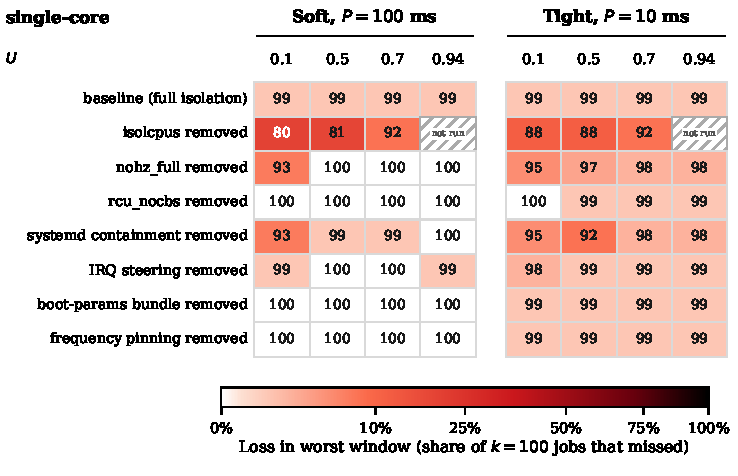
\includegraphics[width=\textwidth]{figures_RQ1/worst_window_k100_heatmap_single-core.pdf}
\caption{Worst window of $k = 100$ consecutive jobs for every configuration, period scale and utilization, single-core. Each cell gives $m$, the smallest number of jobs that met their deadline in any window of 100 jobs. Cells with $m = 100$ have no colour; the more jobs missed, the more intense the red, and black means that every job of the window missed. The colour follows the loss $(k-m)/k$ on a \emph{square-root} scale, so that small losses stay distinguishable from zero. Hatched cells were not run.}
\label{fig:worst-window-k100-heatmap-single-core}
\end{figure}
